\chapter{DESARROLLO\label{sec:desarrollo}}

\clearpage

El desarrollo de la solución software, que ya sabemos que va a ser una aplicación web de mensajería instantánea, se puede explicar en los siguientes apartados que están ordenados según el avance de dicho desarrollo.

\section{Diseño del protocolo de mensajería instantánea}

El protocolo de mensajería instantánea debe permitir que dos o más usuarios en una misma sala envíen mensajes entre ellos y que estos mensajes están identificados por el usuario de quien lo envió. Además, cuando un nuevo usuario entra o un usuario ya en sala sale, el protocolo debe definir también como notifica a los usuarios que están en la sala de que la lista de participantes de la sala ha cambiado.

\subsection{Mensajes JSON del protocolo}

En primer lugar, vamos a comentar los mensajes (JSON) que se han definido para este protocolo y su papel.

\begin{figure}[htp!]
  \centering
  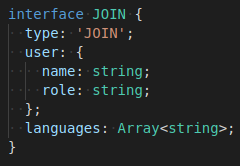
\includegraphics[scale=0.5,clip=true]{ws_join}
  \caption{Interfaz del mensaje de tipo JOIN}
  \label{fig:ws_join}
\end{figure}

Tenemos el primer mensaje de todos, el mensaje JOIN. Con este mensaje un usuario nuevo, que ha conseguido establecer una conexión WebSocket, notifica al servidor con qué credenciales o información de usuario debe autenticar la sesión WebSocket. Por ello, contiene un nombre de usuario, el rol en la sala y una lista de idiomas que entiende el usuario.

\begin{figure}[htp!]
  \centering
  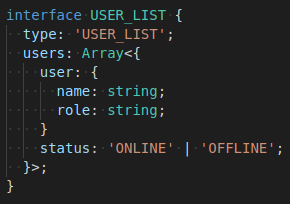
\includegraphics[scale=0.5,clip=true]{ws_user_list}
  \caption{Interfaz del mensaje de tipo USER\_LIST}
  \label{fig:ws_user_list}
\end{figure}

Por otro lado, el servidor debe notificar a los usuarios de que un nuevo usuario ha entrado en la sala. Esto lo consigue con el mensaje USER\_LIST, el cual contiene la lista de usuarios actuales en la sala

Este mensaje también se envía cuando un usuario ha salido de la sala.

Por último, respecto a los mensajes, tenemos el mensaje TEXT\_MESSAGE. Este mensaje lo envía un usuario con el contenido del mensaje en sí junto al idioma en el que lo escribió.

\begin{figure}[htp!]
  \centering
  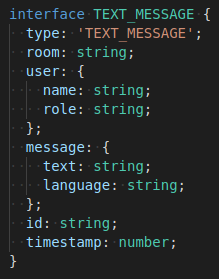
\includegraphics[scale=0.5,clip=true]{ws_text_message}
  \caption{Interfaz del mensaje de tipo TEXT\_MESSAGE}
  \label{fig:ws_text_message}
\end{figure}

Cuando el servidor lo recibe, rellena más campos como quien ha realizado el mensaje, sala en donde se envio y lo reenvía a todos los participantes de dicha sala, incluido el emisor del mensaje.

\subsection{Fases del protocolo}

En este protocolo podemos diferenciar tres fases: entrar en la sala, enviar mensajes de texto y salir de la sala.

\subsubsection{Entrar en la sala}

En esta fase, el usuario una vez conectado al servidor WebSocket envía el mensaje JOIN previamente visto y espera la respuesta USER\_LIST con la lista actual de usuarios en la sala. En esta lista debe aparecer él también, ya que ahora es un participante más de la sala.

En el caso de que otro usuario entrase después que él, este nuevo usuario genera un mensaje USER\_LIST para todos los participantes. De esta forma, el primer usuario y el otro usuario, conocen realmente quienes están en la sala.

\begin{figure}[htp!]
  \centering
  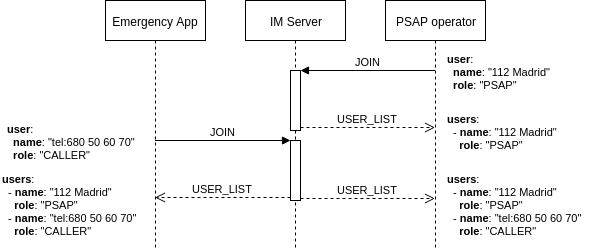
\includegraphics[scale=0.6,clip=true]{im_join_fase}
  \caption{Fase inicial del protocolo IM}
  \label{fig:im_join_fase}
\end{figure}

\subsubsection{Enviar mensajes de texto}

En esta fase, el usuario ya puede enviar mensajes de texto a través del mensaje TEXT\_MESSAGE. Cuando el usuario envio un mensaje de este tipo, el servidor lo trata y si todo va bien, lo reenvía a todos los participantes de la sala, incluido este usuario, con un campo extra que indica quién fue el emisor del mensaje.

\begin{figure}[htp!]
  \centering
  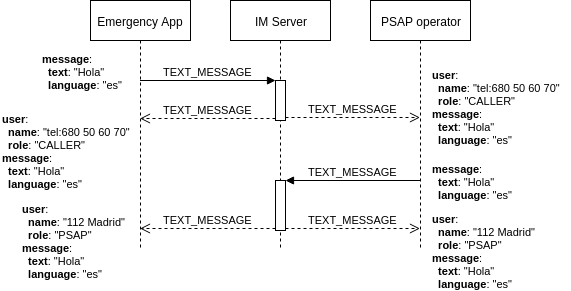
\includegraphics[scale=0.6,clip=true]{im_protocolo_fase_send}
  \caption{Fase de intermedio del protocolo IM}
  \label{fig:im_protocolo_fase_send}
\end{figure}

\subsubsection{Salir de la sala}

En esta fase, el usuario desea salir de la sala y para ello solo le hace falta cerrar la sesión WebSocket. Cuando el servidor se percata de que un cliente WebSocket ha sido cerrado, envia al resto de participantes, si los hay, un mensaje USER\_LIST con la lista actualizada; es decir, sin el usuario que ha salido.

\begin{figure}[htp!]
  \centering
  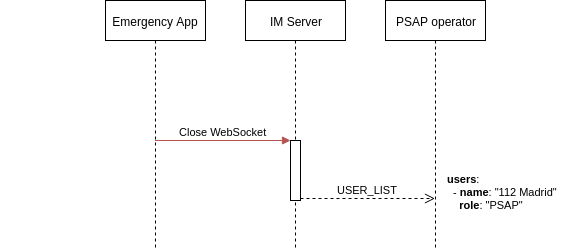
\includegraphics[scale=0.6,clip=true]{im_fase_cierre}
  \caption{Fase de final del protocolo IM}
  \label{fig:im_fase_cierre}
\end{figure}

\section{Diseño del modelo de la base de datos}

El modelo de la base de datos tiene que aprovechar las ventajas de una base de datos NoSQL. Por lo tanto, en vez de pensar en un modelo donde cada recurso ocupa una nueva tabla, hay que pensar en el recurso principal del cual otros recursos (o colecciones) pueden depender. Estas dependencias pueden estar (auto) incluidas en la misma estructura del recurso. Mejorando de este modo las operaciones de lectura y escrita que ofrecen este tipo de base de datos.

Teniendo en cuenta esto, el recurso principal es la sala (room). Y la estructura contiene lo siguiente:

\begin{itemize}
  \item \textbf{Nombre de la sala}. Identificador único que se autogenera y se usa para generar los enlaces a la salas.
  \item \textbf{Token del usuario}. Es el token que el usuario ha usado para crear dicha sala. Su función es relevante si el usuario necesita recuperar en el enlace a la sala.
  \item \textbf{Lista de usuarios}. Son los usuarios que pertenecen a esta sala.
  \item \textbf{Lista de mensajes}. Son los mensajes que los usuarios han enviado. Para la primera versión no haría falta, ya que no se busca tener un historial de la conversación.
\end{itemize}

\begin{figure}[htp!]
  \centering
  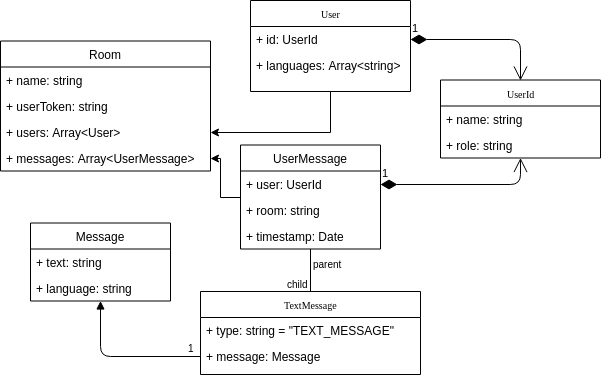
\includegraphics[scale=0.5,clip=true]{im_db}
  \caption{Modelos del IM}
  \label{fig:im_db}
\end{figure}

Como se puede observar en la figura, los subdocumentos de una sala también tiene una estructura predefinida.

El subdocumento User tiene los siguientes campos:

\begin{itemize}
  \item \textbf{Identificador de usuario}. Este identificador es un objeto compuesto por el nombre del usuario y el rol que tiene en la sala.
  \item \textbf{Idiomas}. Es una lista que contiene los idiomas que el usuario maneja. Como en una primera versión, el protocolo solo admite mensajes de texto, podemos asumir que esos idiomas son los que él sabría leer correctamente.
\end{itemize}

Respecto al subdocumento UserMessage, hay que resaltar que su estructura sirve como base para que otras estructuras usen un campo que identifique el tipo de estructura (discriminator, como lo llaman en las bases de datos NoSQL). Este campo, por ejemplo, en nuestro caso sirve para distinguir mensajes de tipo TEXT\_MESSAGE. Pero imaginemos que un futuro, el protocolo admite nuevos tipos de mensajes cómo TRANSLATION o REPLY.

El subdocumento TextMessage tiene los siguientes campos:

\begin{itemize}
  \item \textbf{Tipo de mensaje de usuario}. Identifica que es de tipo TextMessage añadiendo el valor TEXT\_MESSAGE.
  \item \textbf{Mensaje del usuario}. Es un objeto compuesto por el mensaje de texto del usuario y el idioma en el que debería estar escrito.
\end{itemize}

\section{Diseño de la arquitectura de la aplicación web}

Como ya hemos visto, la aplicación web debe cumplir el protocolo que previamente hemos definido para la mensajería instantánea. Ya sabemos que vamos a tener usuarios por parte de las apps para emergencias y usuarios desde el PSAP que esta atiendo esas llamadas solicitando crear salas. También tenemos claro que la aplicación tiene acceso a una base de datos para tener persistencia de las salas. Y, por último, en las salas los usuarios estarán conectados por WebSocket enviando mensajes de texto entre ellos.

\begin{figure}[htp!]
  \centering
  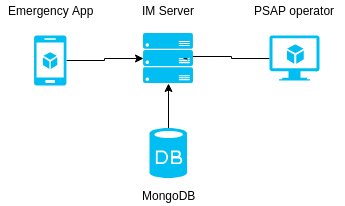
\includegraphics[scale=0.6,clip=true]{im_apps}
  \caption{Infraestructura del servicio IM}
  \label{fig:im_apps}
\end{figure}

Por lo que, ahora hay que centrarse en definir los diferentes módulos que hace esto posible. Y cómo interactúan unos con otros.

Podemos destacar tres principales módulos, que trabajan en conjunto dentro de la aplicación web. Estos módulos son:

\begin{figure}[htp!]
  \centering
  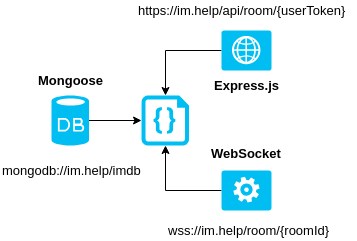
\includegraphics[scale=0.6,clip=true]{im_componentes}
  \caption{Estructura de la aplicación web}
  \label{fig:im_componentes}
\end{figure}

\begin{itemize}
  \item \textbf{Mongoose}. Este módulo se encarga de las operaciones con la base de datos. Habla con la API REST para crear salas y gestiona las operaciones también de los clientes WebSocket.
  \item \textbf{Express.js}. Este módulo se encarga de las rutas a las API de los recursos de la aplicación. En nuestro caso, solo hay un recurso expuesto, las salas. También configura los middlewares y el tratamiento de errores durante la ejecución.
  \item \textbf{WebSocket}. Este módulo se encarga de los clientes WebSocket. Habla con Mongoose para saber si las rutas a las salas siguen existiendo y gestiona los recursos de memoria que se usan en las conexiones WebSocket.
\end{itemize}

\section{Desarrollo del servidor REST}

La aplicación web también tiene API REST para la gestión de los recursos que permitimos que los usuarios puedan manipularlos. En nuestro caso, según el diseño previo, solo los usuarios pueden acceder al recurso sala (room internamente en la aplicación).

\subsection{API de las salas}

Esta API se encarga de manipular el recurso sala dentro de la aplicación. Define los método, READ, CREATE, UPDATE o DELETE, que podemos hacer sobre este recurso. Pero en nuestro caso, solo vamos a permitir CREATE.

\begin{figure}[htp!]
  \centering
  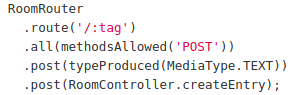
\includegraphics[scale=0.5,clip=true]{room_router}
  \caption{Router de la Room API}
  \label{fig:room_router}
\end{figure}

Por lo que solo debemos añadir el controlador de las salas que solo admite peticiones POST en la ruta \textbf{/api/room/:tag}.

\subsubsection{Crear una sala}

Cuando el servidor web recibe una petición POST sobre la ruta \textbf{/api/room/:tag}, indica al controlador de salas que gestione esta petición. Este controlador al ver que es una petición POST, lo trata como una operación de creación de sala. Por lo que realiza las siguientes actividades:

\begin{figure}[htp!]
  \centering
  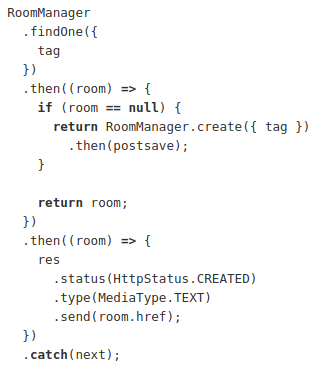
\includegraphics[scale=0.5,clip=true]{rest_room}
  \caption{Acción de crear sala}
  \label{fig:rest_room}
\end{figure}

\begin{enumerate}
  \item \textbf{Extrae el token del usuario de la ruta}. A diferencia de una acción CREATE de una API REST de toda la vida, esta recibe un parámetro de ruta (obligatorio) que le permite al usuario recuperar la sala creada previamente. Evitando de este modo que se cree una nueva sala, en el caso de que perdiese el enlace del WebSocket de la sala.
  \item \textbf{Busca la sala en la base de datos}. Cada sala tiene asociado un token de usuario único, por lo que el controlador buscará dicha sala a partir de este token.
  \item \textbf{Crear nueva sala}. En el caso de que no se encuentra la sala, el controlador creará una nueva sala a partir de ese token dado.
  \item \textbf{Enviar enlace de la sala}. De un modo u otro, el controlador envía el enlace de la sala (HTTP) como cuerpo de la respuesta. Como es una API REST, la respuesta también un 201 indicando que la petición de creación/recuperación de sala ha ido con éxito.
\end{enumerate}

Una vez que el usuario que ha realizado la petición de creación de sala, recibe el enlace a la nueva sala ya puede unirse a ella cuando desee.

\begin{figure}[htp!]
  \centering
  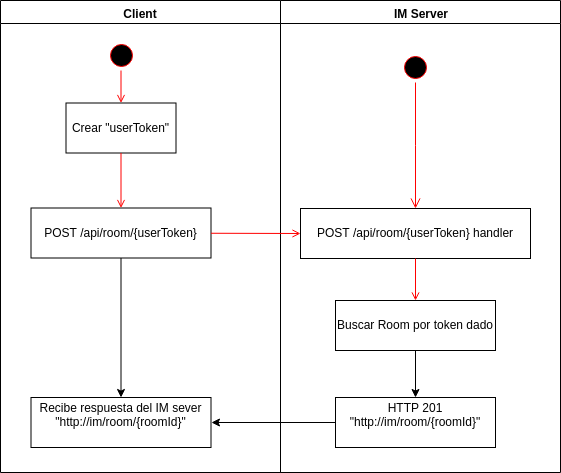
\includegraphics[scale=0.5,clip=true]{room_post}
  \caption{Flujo de creación de sala}
  \label{fig:room_post}
\end{figure}

\section{Desarrollo del servidor WebSocket}

La aplicación web también debe atender conexiones WebSocket. En este apartado vamos a ver qué actividades realiza el servidor WebSocket cuando ocurre las siguientes situaciones.

\subsection{Conexión de un cliente WebSocket}

Cuando se establece una nueva conexión WebSocket, el servidor realiza las siguientes actividades:

\begin{enumerate}
  \item \textbf{Validar de la ruta}. La ruta de la URL del WebSocket tiene que coincidir con \textbf{/room/\{roomId\}}. En caso de que no case, se cierra la conexión.
  \item \textbf{Buscar la sala}. Se extrae el identificador de la sala, y se usa para buscar en la base de datos dicha sala. En caso de no encontrarla, se cierra la conexión.
  \item \textbf{Aceptar conexión temporal}. El cliente WebSocket es válido de momento. El servidor queda a la espera de un mensaje JOIN por parte del nuevo cliente. Si no se recibe dicho mensaje en un determinado tiempo, se cierra la conexión.
\end{enumerate}

\subsection{Tratamiento de los mensajes JOIN}

Si el cliente WebSocket ha enviado un mensaje JOIN, el servidor realiza las siguientes actividades:

\begin{enumerate}
  \item \textbf{Validar el mensaje JOIN}. El mensaje de texto recibido se deserializa a un objeto JavaScript para luego validarlo. Si la estructura no coincide con un mensaje JOIN, se cierra la conexión.
  \item \textbf{Buscar el usuario}. El servidor extrae la información del usuario contenida en el mensaje JOIN y luego busca si ese usuario ya existía en la sala. En caso de que no exista, se crea una nueva entrada en la lista de usuarios de la sala almacenada en la base de datos.
  \item \textbf{Autenticar la session}. El cliente WebSocket ahora tiene asociado el usuario que mandó previamente.
  \item \textbf{Difundir nuevo usuario en sala}. Ahora hay un nuevo usuario en la sala, por lo que el servidor envía a todos los participantes, incluido el nuevo usuario, el mensaje USER\_LIST con la lista de usuarios actualizada.
\end{enumerate}

\subsection{Tratamiento de los mensajes TEXT\_MESSAGE}

Ahora, el cliente WebSocket es un participante más de la sala y envía un mensaje TEXT\_MESSAGE. El servidor realiza las siguientes actividades:

\begin{enumerate}
  \item \textbf{Validar el mensaje TEXT\_MESSAGE}. El mensaje de texto recibido se deserializa a un objeto JavaScript para luego validarlo. Si la estructura no coincide con un mensaje TEXT\_MESSAGE, se descarta.
  \item \textbf{Actualizar la lista de mensajes de la sala}. El servidor extrae la información del mensaje del usuario contenida en el mensaje TEXT\_MESSAGE y lo añada a la lista de mensajes de sala en la base de datos.
  \item \textbf{Difundir el nuevo mensaje}. El servidor envía a todos los participantes, incluido el emisor del mensaje, el mensaje TEXT\_MESSAGE con el mensaje del usuario.
\end{enumerate}

\subsection{Desconexión de un cliente WebSocket}

El protocolo de IM definido para esta aplicación, no incluye algún tipo de mensaje para que el usuario indique que quiere abandonar la sala. Pero no es necesario, con que el cliente WebSocket cierre la conexión es más que suficiente. Cuando sucede esto, el servidor realiza las siguientes actividades:

\begin{enumerate}
  \item \textbf{Comprobar si está autenticado}. El servidor no sabe, si la desconexión viene del temporizador que espera un primer mensaje JOIN que nunca llegó o que el cliente ha decidido cerrar la conexión. Por lo tanto, es necesario comprobar si la sesión tiene un usuario para luego borrarlo.
  \item \textbf{Actualizar la lista de usuarios de la sala}. El servidor actualiza la lista de usuarios de la sala, borrando el usuario de la sesión.
  \item \textbf{Difundir el nuevo mensaje}. El servidor envía a todos los participantes restantes de la sala, el mensaje USER\_LIST con la lista de usuarios actualizada.
\end{enumerate}

\section{Creación de la imagen para Docker}

Ahora que tenemos funcionando la aplicación web, es ahora de crear la imagen para Docker.

Para ello, creamos en primer lugar el fichero \textbf{Dockerfile} en la carpeta raíz de la aplicación y definimos las siguientes instrucciones dentro de él:

\begin{enumerate}
  \item \textbf{Definir imagen base}. Especificar qué imagen base debe Docker, desde la que se crea el contenedor Docker y para la que Node.js, en nuestro caso, ejecute las siguientes instrucciones del Dockerfile posteriormente. Elegimos la última versión LTS de Node.js, por ejemplo.
  \item \textbf{Configurar directorio por defecto}. Indicamos la ruta del directorio donde tener pensado ejecutar los siguientes comandos que instalan y configuran nuestra aplicación.
  \item \textbf{Instalar paquetes Node.js}. Especificamos qué paquetes debe instalar dentro de la imagen.
  \item \textbf{Copiar la aplicación web}. Especificamos los ficheros fuente que debe añadir dentro de la imagen.
  \item \textbf{Exponer puertos}. Muestramos los puertos que se exponen en el contenedor Docker. Podemos especificar varios puertos de contenedor, pero en nuestro caso solo es necesario uno, 3000, que es donde por defecto se encuentra escuchando el servidor web.
  \item \textbf{Comando inicial del contenedor}. Especificamos el ejecutable (node) y los parámetros predeterminados (aplicación y puerto), que se combinan en el comando que el contenedor ejecuta en el momento del lanzamiento.
\end{enumerate}

\begin{figure}[htp!]
  \centering
  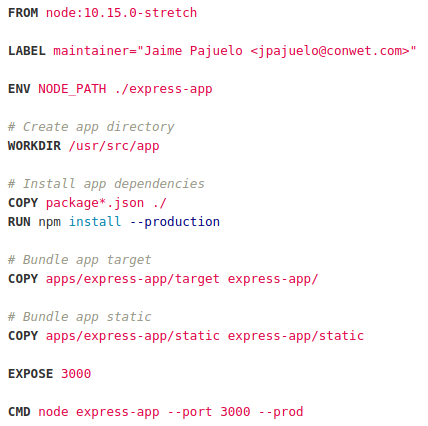
\includegraphics[scale=0.5,clip=true]{dockerfile}
  \caption{Contenido del Dockerfile}
  \label{fig:dockerfile}
\end{figure}

\section{Desarrollo del entorno de pruebas de rendimiento}

El este apartado sigue la metodología de pruebas de rendimiento que hay que seguir para el diseño de un entorno de pruebas según Microsoft Developer Network.

\subsection{Identificar el entorno de pruebas}

En esta fase se identifica el entorno físico del plan de pruebas y el entorno de la aplicación web, así como las herramientas y recursos de que dispone el equipo de prueba. Tener desde el principio un profundo conocimiento de todo el entorno de pruebas permite diseños de pruebas más eficientes \cite{jmeter6}.

En el entorno del plan de pruebas se destaca lo siguiente:

\begin{itemize}
  \item Ubuntu 18.10: sistema operativo de distribución GNU/Linux.
  \item Apache Maven 3.6.1: herramienta software para la gestión de paquetes de un proyecto Java.
  \item OpenJDK 11: versión libre del SDK de Java.
\end{itemize}

Y, por el otro lado, en el entorno de la aplicación web:

\begin{itemize}
  \item Ubuntu 18.10: sistema operativo de distribución GNU/Linux.
  \item NPM 6.4.1: gestor de paquetes JavaScript de Node.js.
  \item Node.js 10.16.0 LTS: entorno de ejecución para JavaScript.
\end{itemize}

\subsection{Identificar los criterios de aceptación de rendimiento}

En esta fase se determina el tiempo de respuesta, el rendimiento, la utilización de los recursos y los objetivos y limitaciones. En general, el tiempo de respuesta concierne al usuario, el rendimiento de la capa de negocio, y la utilización de los recursos al sistema.

Identificar cuáles serían criterios de éxito de rendimiento del proyecto para evaluar qué combinación de la configuración da lugar a un funcionamiento óptimo \cite{jmeter6}.

Teniendo en cuenta que el servicio de mensajería instantánea es una funcionalidad que será accesible a los usuarios una vez que el operador lo haya visto oportuno. Es decir, que el número de peticiones al servidor web está limitado por el número del personal del PSAP en cuestión.

Es una ventaja, ya que tenemos un escenario bastante favorable para nuestra aplicación web. Por lo tanto, la aplicación web debe estar disponible siempre que el operador lo solicite. El tiempo de respuesta debe ser óptimo ya que se encuentra en sistema de emergencia.

\subsection{Planificar y diseñar las pruebas}

En esta fase se identifica los principales escenarios, se determina la variabilidad de los usuarios y la forma de simular esa variabilidad, se define los datos de las pruebas y se establecen las métricas a recoger \cite{jmeter6}.

En el capítulo anterior, hemos visto las métricas del centro 112 de Madrid las cuales nos puede servir para definir los diferentes escenarios de las pruebas.

El escenario principal consiste en:

\begin{enumerate}
  \item El operador solicita al cliente de mensajería instantánea una sala de IM vacía.
  \item El operador se une a esa sala y envía el enlace al usuario.
  \item El usuario se une también a la sala.
  \item Ambos participantes empiezan a enviar mensajes.
  \item Ambos salen de las sala, y pasado un tiempo esta sala se elimina.
\end{enumerate}

Como el centro 112 de Madrid tiene a su disposición como unos 250 profesionales en la atención de llamadas, podríamos fijar ese número como el punto intermedio de la variabilidad de las salas simultáneas.

Como se trata de una llamada entre un ciudadano y un operador, el número mínimo de usuarios por sala debe ser 2. En ocasiones, otro personal del PSAP participan en la llamada como la policía, los bomberos o la asistencia médica, además de otros profesionales, como intérpretes. Por lo tanto, supongamos el peor caso como punto intermedio de la variabilidad de los usuarios por sala simultáneos; es decir que se encuentren todos participando en la misma sala, saldría unos 5.

El centro 112 de Madrid tiene un tiempo medio de respuesta de 8 segundos y un tiempo medio de resolución de la emergencia de 70 segundos. Estos valores pueden ser útiles para saber cuánto tiempo tenemos para crear una sala y que dos personas como mínimo se encuentren en ella, y también, la duración media de una conversación en la sala.

Finalmente, el plan de pruebas se define del siguiente modo:

\begin{enumerate}
  \item Dado un número de salas, un número de usuarios por sala y una frecuencia de envío de mensajes como parámetros de entrada.
  \item Dado el tiempo de duración de la prueba y la dirección de donde se encuentra la aplicación web como variables de entorno.
  \item Se crean el número de salas dado.
  \item Se lanzan grupos de threads (salas) que contengan cada uno el número de usuarios por sala dado.
  \item Cada thread se conecta al websocket de la sala y envía un mensaje que quiere unirse a la sala.
  \item Una vez que sepa que está dentro de la sala, empieza a enviar mensajes con la frecuencia de envío de mensajes dada.
  \item Cuando pasa el tiempo de duración de la prueba, todos los threads se cierran.
  \item Y se recogen los resultados.
\end{enumerate}

Los resultados se exportan a un fichero CSV con el siguiente formato: sala, usuario, tipo de mensaje y tiempo de respuesta.

Los variabilidad de los datos de entrada son:

\begin{itemize}
  \item Número de salas: 1 al 10 con salto 1, del 20 al 100 con salto 10, y del 200 al 500 con salto 100.
  \item Número de salas por usuario: 1 al 20 con salto 2.
  \item Frecuencia de envío de mensajes: 0,2 al 2 con salto 0,2.
\end{itemize}

\subsection{Configurar el entorno de prueba}

En esta fase se prepara el entorno de prueba, las herramientas y recursos necesarios para ejecutar cada una de las estrategias, así como las características y componentes disponibles para la prueba. Asegurarse de que el entorno de prueba se ha preparado para la monitorización de los recursos según sea necesario \cite{jmeter6}.

En el entorno de prueba se ha instalado OpenJDK 11 y Maven utilizando aptitude de Ubuntu. También se descargado el binario de la última versión de Eclipse disponible para el desarrollo del plan de pruebas en Java.

Y se ha configurado la JVM para que cada thread tenga más espacio para realizar sus peticiones y pueda almacenar los resultados sin problemas.

\begin{figure}[htp!]
  \centering
  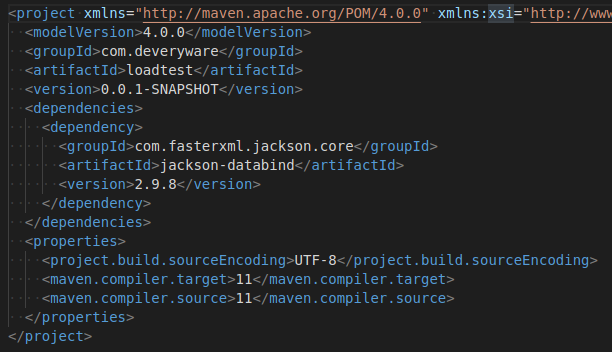
\includegraphics[scale=0.5,clip=true]{pom}
  \caption{Fichero pom.xml}
  \label{fig:pom}
\end{figure}

\begin{figure}[htp!]
  \centering
  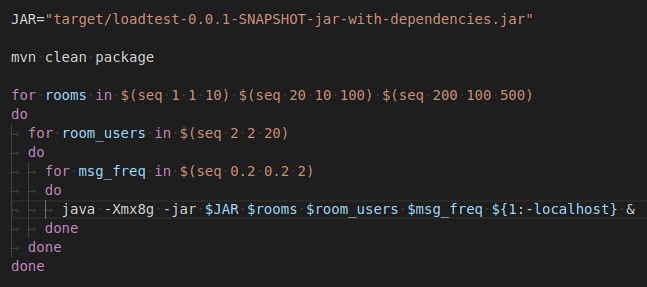
\includegraphics[scale=0.5,clip=true]{test_bash}
  \caption{Script para ejecutar el plan de pruebas}
  \label{fig:test_bash}
\end{figure}

\subsection{Aplicar el diseño de la prueba}

En esta fase se desarrolla las pruebas de rendimiento de acuerdo con el diseño del plan \cite{jmeter6}.

Para ello creamos un proyecto Java a partir del \textbf{pom.xml}, y definimos las siguientes clases:

\begin{itemize}
  \item \textbf{TestPlan}. Esta clase recibe como parámetros de entrada la dirección de la aplicación web, el número de salas que debe crear, el número de usuarios (threads) que debe crear por cada sala y el periodo de envío de mensajes. Su cometido es crear las salas, crear los threads, y esperar que los threads acaben en un determinado tiempo para recoger los resultados de cada thread.
  \item \textbf{User}. Esta es la clase que representa a un usuario que decide conectarse a una sala dada y realizar todo el proceso del protocolo de IM. Por ello, necesita saber qué nombre usar como el mensaje JOIN, la dirección del WebSocket de la sala y el periodo de envío de mensajes. También recibe una variable boolean, que es compartida por otros User, que indica cuando deben cerrar la conexión WebSocket y devolver los resultados de la prueba.
  \item \textbf{ThreadResult}. Se encarga de recoger los tiempos de respuesta etiquetados de un determinado usuario.
  \item \textbf{ResponseTime}. Esta clase representa un tiempo de respuesta etiquetado. La etiqueta es el tipo de mensaje que se envió al servidor, JOIN o TEXT\_MESSAGE.
\end{itemize}

\begin{figure}[htp!]
  \centering
  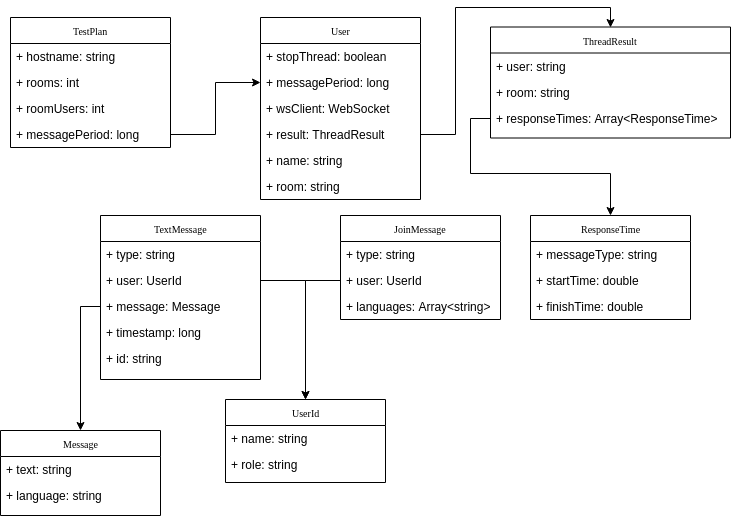
\includegraphics[scale=0.5,clip=true]{testplan}
  \caption{Diagrama de clases del entorno de pruebas}
  \label{fig:testplan}
\end{figure}

Ahora, creamos la función principal del plan de pruebas. La cual espera recibir el número de salas, el número de usuarios de por sala, la frecuencia de envío de mensajes y la dirección de la aplicación web.

Una vez termina el plan de pruebas, esta también se encarga de almacenar todos los resultados de la prueba en un fichero CSV. Este fichero CSV indica en su propio nombre los parámetros con los que fue ejecutado.

\begin{figure}[htp!]
  \centering
  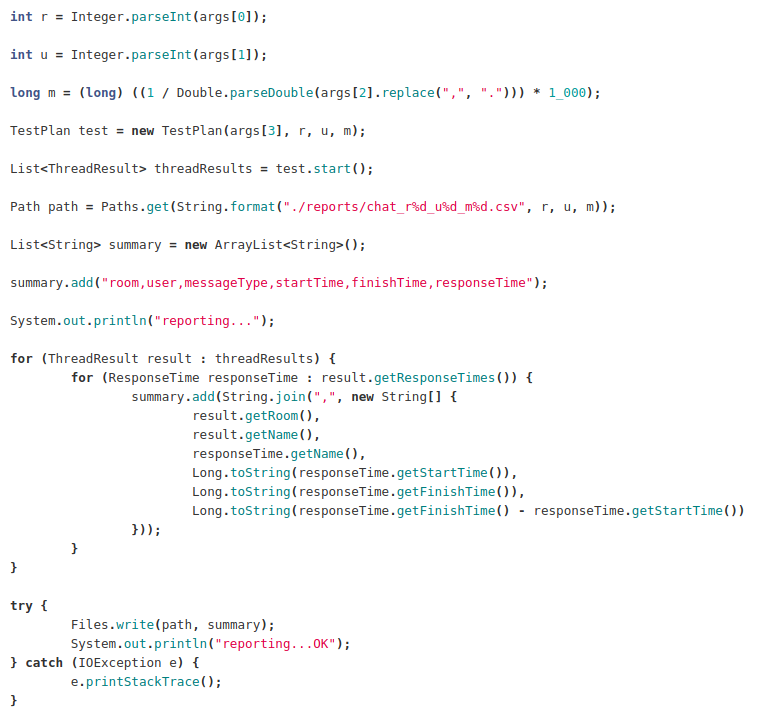
\includegraphics[scale=0.5,clip=true]{load_main}
  \caption{Función principal de la prueba de rendimiento}
  \label{fig:load_main}
\end{figure}

El resto de clases como TextMessage, JoinMessage, Message o UserId sirven para la serialización o deserialización de los mensajes JSON que se envían durante la conexión WebSocket.

\begin{figure}[htp!]
  \centering
  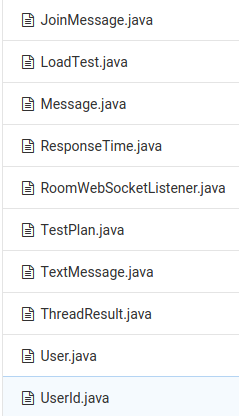
\includegraphics[scale=0.5,clip=true]{testplan_app}
  \caption{Estructura del entorno de pruebas}
  \label{fig:testplan_app}
\end{figure}
